\documentclass[journal,10pt,twocolumn]{article}
\usepackage{graphicx}
\usepackage[margin=0.5in]{geometry}
\usepackage[cmex10]{amsmath}
\usepackage{array}
\usepackage{booktabs}
\usepackage{mathtools}
\title{\textbf{Optimization Assignment - 2}}
\author{Alavala Chinnapa Reddy}
\date{September 2022}


\providecommand{\norm}[1]{\left\lVert#1\right\rVert}
\providecommand{\abs}[1]{\left\vert#1\right\vert}
\let\vec\mathbf
\newcommand{\myvec}[1]{\ensuremath{\begin{pmatrix}#1\end{pmatrix}}}
\newcommand{\mydet}[1]{\ensuremath{\begin{vmatrix}#1\end{vmatrix}}}
\providecommand{\brak}[1]{\ensuremath{\left(#1\right)}}
\providecommand{\lbrak}[1]{\ensuremath{\left(#1\right.}}
\providecommand{\rbrak}[1]{\ensuremath{\left.#1\right)}}
\providecommand{\sbrak}[1]{\ensuremath{{}\left[#1\right]}}

\begin{document}

\maketitle
\paragraph{\textit{Problem Statement} - Find the maximum and minimum values of $f (x) = (2x – 1)^2+ 3$. }
\section*{\large Solution}
\subsection*{\normalsize Gradient descent}
Let 
\begin{align}
	f(x) = (2x-1)^2+3\\
	\implies f(x) = 4x^2-4x+4
	\label{eq:quad_exp}
\end{align}
\begin{eqnarray}
(2x-1)^2\geq0\\
f(x)\geq3\\
	\boxed{\text{Maxima}=\infty}
\end{eqnarray}
f(x)  consists only minima,\\

Using gradient ascent method we can find its minima ,
    \begin{align}
        x_{n+1} &= x_n - \alpha \nabla f(x_n) \\
        \implies x_{n+1} &= x_n - \alpha \brak{8x_n-4}
    \end{align}
    
Taking $x_0=0.1,\alpha=0.001$ and precision = 0.00000001, values obtained using python are:
    
    \begin{align}
        \boxed{\text{Minima} = 3.00000}\\
        \boxed{\text{Minima Point} = 0.50000}
    \end{align}

\begin{figure}[t]
	\centering
	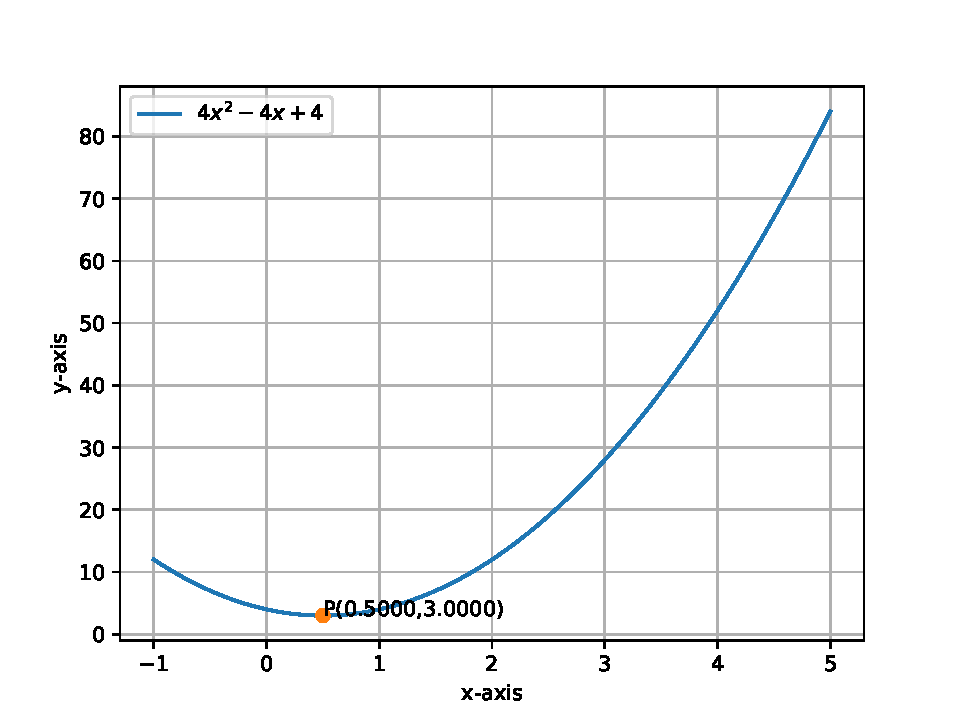
\includegraphics[width=1\columnwidth]{figs/2.pdf}
	\caption{Graph of $f(x)$ in \eqref{eq:quad_exp}}
	\label{fig:graph_fx}
\end{figure}

\end{document}
